\documentclass[landscape,twocolumn,letterpaper,9pt,reqno]{article}\usepackage[]{graphicx}\usepackage[]{color}
%% maxwidth is the original width if it is less than linewidth
%% otherwise use linewidth (to make sure the graphics do not exceed the margin)
\makeatletter
\def\maxwidth{ %
  \ifdim\Gin@nat@width>\linewidth
    \linewidth
  \else
    \Gin@nat@width
  \fi
}
\makeatother

\definecolor{fgcolor}{rgb}{0.345, 0.345, 0.345}
\newcommand{\hlnum}[1]{\textcolor[rgb]{0.686,0.059,0.569}{#1}}%
\newcommand{\hlstr}[1]{\textcolor[rgb]{0.192,0.494,0.8}{#1}}%
\newcommand{\hlcom}[1]{\textcolor[rgb]{0.678,0.584,0.686}{\textit{#1}}}%
\newcommand{\hlopt}[1]{\textcolor[rgb]{0,0,0}{#1}}%
\newcommand{\hlstd}[1]{\textcolor[rgb]{0.345,0.345,0.345}{#1}}%
\newcommand{\hlkwa}[1]{\textcolor[rgb]{0.161,0.373,0.58}{\textbf{#1}}}%
\newcommand{\hlkwb}[1]{\textcolor[rgb]{0.69,0.353,0.396}{#1}}%
\newcommand{\hlkwc}[1]{\textcolor[rgb]{0.333,0.667,0.333}{#1}}%
\newcommand{\hlkwd}[1]{\textcolor[rgb]{0.737,0.353,0.396}{\textbf{#1}}}%
\let\hlipl\hlkwb

\usepackage{framed}
\makeatletter
\newenvironment{kframe}{%
 \def\at@end@of@kframe{}%
 \ifinner\ifhmode%
  \def\at@end@of@kframe{\end{minipage}}%
  \begin{minipage}{\columnwidth}%
 \fi\fi%
 \def\FrameCommand##1{\hskip\@totalleftmargin \hskip-\fboxsep
 \colorbox{shadecolor}{##1}\hskip-\fboxsep
     % There is no \\@totalrightmargin, so:
     \hskip-\linewidth \hskip-\@totalleftmargin \hskip\columnwidth}%
 \MakeFramed {\advance\hsize-\width
   \@totalleftmargin\z@ \linewidth\hsize
   \@setminipage}}%
 {\par\unskip\endMakeFramed%
 \at@end@of@kframe}
\makeatother

\definecolor{shadecolor}{rgb}{.97, .97, .97}
\definecolor{messagecolor}{rgb}{0, 0, 0}
\definecolor{warningcolor}{rgb}{1, 0, 1}
\definecolor{errorcolor}{rgb}{1, 0, 0}
\newenvironment{knitrout}{}{} % an empty environment to be redefined in TeX

\usepackage{alltt}

\usepackage{lscape,fancyhdr}

\usepackage{hyperref}
\usepackage{float}
\pagestyle{fancy}

\usepackage{amsmath,epsfig,subfigure,amsthm,amsfonts,epsf,psfrag,rotating,setspace,bm}

\usepackage{verbatim,color} % Allow text colors}

\setlength{\oddsidemargin}{-0.4in}		% default=0in
\setlength\evensidemargin{-0.4in}

\setlength{\textwidth}{9.8in}		% default=9in

\setlength{\columnsep}{0.5in}		% default=10pt

\setlength{\columnseprule}{0pt}		% default=0pt (no line)


\setlength{\textheight}{7.0in}		% default=5.15in

\setlength{\topmargin}{-0.75in}		% default=0.20in

\setlength{\headsep}{0.25in}		% default=0.35in

\setlength{\parskip}{1.2ex}

\setlength{\parindent}{0mm}

\lhead{Course EPIB607: Regression handout 006 (Logistic regression - HIV and Smoking examples)}
\rhead{jh,sb \ \ \ v. 2018.11.26}
\IfFileExists{upquote.sty}{\usepackage{upquote}}{}
\begin{document}
	


\section{Cesarean section and transmission of HIV}

\vspace{-0.1in}

To evaluate the relation between elective cesarean section and vertical (mother-to-child) transmission of human immunodeficiency virus type 1 (HIV-1), the authors performed a meta-analysis using data on individual patients from 15 prospective cohort studies.

\begin{figure}[h]
	\centering
	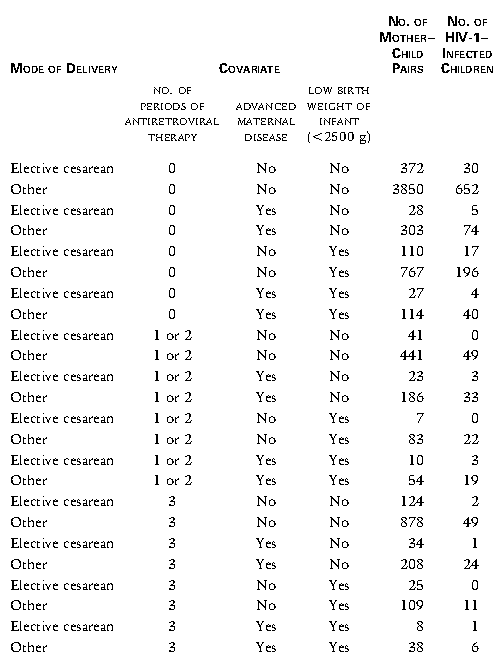
\includegraphics[scale=1.1]{hivtable.pdf}
\end{figure}




\begin{table}[H]
	\centering
	\begin{tabular}{lcc|c}
			     & Exposed  &   Unexposed & Total  \\		
		Cases    & $a_i$ &  $b_i$ & $M_{1i}$ \\
		Controls & $c_i$ 	& $d_i$  	& $M_{0i}$ 	\\	
		\hline
		Total & $N_{1i}$ & $N_{0i}$ 	& $T_i$
	\end{tabular}
\end{table}


$OR_{MH} = \frac{\sum_i \frac{a_i d_i}{T_i}}{\sum_i \frac{b_i c_i}{T_i}}$ \\ \ \\
$RR_{MH} = \frac{\sum_i \frac{a_i N_{0i}}{T_i}}{\sum_i \frac{b_i N_{1i}}{T_i}}$

\clearpage

\begin{knitrout}\small
\definecolor{shadecolor}{rgb}{0.969, 0.969, 0.969}\color{fgcolor}
\begin{verbatim}
## Call:
## glm(formula = cbind(n.hivpos, n.hivneg) ~ 1, family = binomial(link = logit), 
##     data = ds)
## 
## Coefficients:
##             Estimate Std. Error z value Pr(>|z|)    
## (Intercept)   -1.671      0.031     -54   <2e-16 ***
## ---
## Signif. codes:  0 '***' 0.001 '**' 0.01 '*' 0.05 '.' 0.1 ' ' 1
## 
## (Dispersion parameter for binomial family taken to be 1)
## 
##     Null deviance: 293.95  on 23  degrees of freedom
## Residual deviance: 293.95  on 23  degrees of freedom
## AIC: 387.8
## 
## Number of Fisher Scoring iterations: 4
\end{verbatim}

\end{knitrout}


\begin{knitrout}\small
\definecolor{shadecolor}{rgb}{0.969, 0.969, 0.969}\color{fgcolor}
\begin{verbatim}
## Call:
## glm(formula = cbind(n.hivpos, n.hivneg) ~ caesarian, family = binomial(link = logit), 
##     data = ds)
## 
## Coefficients:
##             Estimate Std. Error z value Pr(>|z|)    
## (Intercept)   -1.606      0.032   -50.2   <2e-16 ***
## caesarian     -0.815      0.132    -6.2    7e-10 ***
## ---
## Signif. codes:  0 '***' 0.001 '**' 0.01 '*' 0.05 '.' 0.1 ' ' 1
## 
## (Dispersion parameter for binomial family taken to be 1)
## 
##     Null deviance: 293.95  on 23  degrees of freedom
## Residual deviance: 247.78  on 22  degrees of freedom
## AIC: 343.7
## 
## Number of Fisher Scoring iterations: 4
\end{verbatim}

\end{knitrout}

\clearpage

\vspace{-0.3in}

\begin{knitrout}\small
\definecolor{shadecolor}{rgb}{0.969, 0.969, 0.969}\color{fgcolor}
\begin{verbatim}
## Call:
## glm(formula = cbind(n.hivpos, ds$n.hivneg) ~ caesarian + ART1or2 + 
##     ART3 + m.advancedHIV + c.LBW, family = binomial(link = logit), 
##     data = ds)
## 
## Coefficients:
##               Estimate Std. Error z value Pr(>|z|)    
## (Intercept)     -1.608      0.041   -39.6   <2e-16 ***
## caesarian       -0.852      0.134    -6.3    2e-10 ***
## ART1or2         -0.362      0.106    -3.4    6e-04 ***
## ART3            -1.178      0.114   -10.3   <2e-16 ***
## m.advancedHIV    0.535      0.090     6.0    3e-09 ***
## c.LBW            0.581      0.075     7.8    9e-15 ***
## ---
## Signif. codes:  0 '***' 0.001 '**' 0.01 '*' 0.05 '.' 0.1 ' ' 1
## 
## (Dispersion parameter for binomial family taken to be 1)
## 
##     Null deviance: 293.945  on 23  degrees of freedom
## Residual deviance:  18.393  on 18  degrees of freedom
## AIC: 122.3
## 
## Number of Fisher Scoring iterations: 4
\end{verbatim}

\end{knitrout}

\vspace{-0.22in}

\begin{knitrout}\small
\definecolor{shadecolor}{rgb}{0.969, 0.969, 0.969}\color{fgcolor}
\begin{verbatim}
## Call:
## glm(formula = cbind(n.hivpos, ds$n.hivneg) ~ caesarian + ART1or2 + 
##     ART3 + m.advancedHIV + c.LBW, family = binomial(link = log), 
##     data = ds)
## 
## Coefficients:
##               Estimate Std. Error z value Pr(>|z|)    
## (Intercept)     -1.793      0.034   -53.2   <2e-16 ***
## caesarian       -0.720      0.119    -6.0    2e-09 ***
## ART1or2         -0.278      0.087    -3.2    0.001 ** 
## ART3            -1.016      0.104    -9.8   <2e-16 ***
## m.advancedHIV    0.409      0.068     6.0    2e-09 ***
## c.LBW            0.453      0.057     7.9    2e-15 ***
## ---
## Signif. codes:  0 '***' 0.001 '**' 0.01 '*' 0.05 '.' 0.1 ' ' 1
## 
## (Dispersion parameter for binomial family taken to be 1)
## 
##     Null deviance: 293.945  on 23  degrees of freedom
## Residual deviance:  21.295  on 18  degrees of freedom
## AIC: 125.2
## 
## Number of Fisher Scoring iterations: 5
\end{verbatim}

\end{knitrout}


\clearpage

\section{Smoking among women in Whickham, UK}
Consider the following \textit{age stratified} mortality data (Rothman, Table 1-2) from a study that looked at smoking habits of residents of Whickham, England, in the period 1972-1974 and then tracked the survival over the next 20 years of those who were interviewed. 


\begin{table}[h]
	\centering
	\begin{tabular}{lcccc}
		 &  &   \multicolumn{2}{c}{Smoking} &  \\		
		Age & Vital Status &  Yes & No & Total \\
		18-24 	& Dead 	& 2  	& 1 	& 3 	\\	
		 		& Alive & 53  	& 61 	& 114 	\\
		 		& Risk & 0.04  	& 0.02 	& 0.03 	\\
		 		\hline
		25-34 	& Dead 	& 3  	& 5 	& 8 	\\	
& Alive & 121  	& 152 	& 273 	\\
& Risk & 0.02  	& 0.03 	& 0.03 \\
\hline 			
35-44 	& Dead 	& 14  	& 7 	& 21 	\\	
& Alive & 95  	& 114 	& 209 	\\
& Risk & 0.13  	& 0.06 	& 0.09 \\
\hline
45-54 	& Dead 	& 27  	& 12 	& 39 	\\	
& Alive & 103  	& 66 	& 169 	\\
& Risk & 0.21  	& 0.15 	& 0.19 \\
		 		\hline
55-64 	& Dead 	& 51  	& 40 	& 91 	\\	
& Alive & 64  	& 81 	& 145 	\\
& Risk & 0.44  	& 0.33 	& 0.39 \\
		 		\hline
65-74 	& Dead 	& 29  	& 101 	& 130 	\\	
& Alive & 7  	& 28 	& 35 	\\
& Risk & 0.81  	& 0.78 	& 0.79 \\
		 		\hline
75+ 	& Dead 	& 13  	& 64 	& 77 	\\	
& Alive & 0  	& 0 	& 0 	\\
& Risk & 1.00  	& 1.00 	& 1.00 \\
\hline
	\end{tabular}
\end{table}










\end{document}
